\documentclass[a4paper]{scrreprt}

\usepackage[ngerman]{babel}
\usepackage[utf8]{inputenc}
\usepackage[T1]{fontenc}
\usepackage{ae}
\usepackage[bookmarks, bookmarksnumbered]{hyperref}
\usepackage{tabularx}
\usepackage{graphicx}
\usepackage{csquotes}
\usepackage{verbatim}
\usepackage[nonumberlist, toc, section]{glossaries}
\usepackage[german]{fancyref}

\makeglossaries

\setcounter{secnumdepth}{4}

\newglossaryentry{Produkt}
{
name=Produkt,
plural=Produkte,
description={Das von uns gelieferte Softwaresystem. Siehe \Gls{Spiel-Server}}
}

\newglossaryentry{Spiel}
{
name=Spiel,
plural=Spiele,
description={Ein Spiel ist eine Instanz eines \Gls{Spielmodus}.
Ein Spiel hat das Ziel das Wissen des Spielers zu nutzen, um die Merkmalsauswahl für Machine-Learning zu unterstützen}
}
\newglossaryentry{Spielmodus}
{
name=Spielmodus,
plural=Spielmodi,
description={Ein Spielmodus ist eine definierte Art und Weise die Merkmalsauswahl durchzuführen. Standardmäßig gibt es die Spielmodi \Gls{Matrix Select} und \Gls{Binar Select}}
}

\newglossaryentry{Spieler}
{
name=Spieler,
plural=Spieler,
description={Eine im System registrierte Person, welche an einem \Gls{Spiel} teilnimmt. Meist ist dies ein Angestellter des Betriebs}
}

\newglossaryentry{Spieleinstellungen}
{
name=Spieleinstellungen,
plural=Spieleinstellungen,
description={Die Einstellungen für ein \Gls{Spiel} umfassen die Art des Spiels, die teilnehmenden \Gls{Spieler} sowie die Endbedingungen des \Gls{Spiel}s}
}
\newglossaryentry{Organisator}
{
name=Organisator,
plural=Organisatoren,
description={Ein Organisator ist eine im System registrierte Person, die neue Spiele erstellt und die Ergebnisse von diesen ausliest}
}
\newglossaryentry{Achievement}
{
name=Achievement,
plural=Achievements,
description={Ein Ziel oder eine Errungenschaft welche den \Gls{Spieler} motiviert weiterzuspielen}
}
\newglossaryentry{Spiel-Server}
{
name=Spiel-Server,
plural=Spiel-Server,
description={Ein Computer, welcher der Verwaltung von CS:Select dient und eine Internetanbindung hat. Dies ist das von uns gelieferte Software-System}
}
\newglossaryentry{ML-Server}
{
name=Machine-Learning-Server,
description={Ein Server, der nicht Bestandteil des \Gls{Produkt}s ist, jedoch benötigt wird, um die Funktionalität des \Gls{Produkt}s herzustellen}
}
\newglossaryentry{Datensatz}
{
name=Datensatz,
plural=Datensätze,
description={Die Menge an Features, die ein Machine-Learning-Modell zur Verfügung hat. Zu jedem Feature gehören eine Beschreibung sowie zwei Grafiken}
}
\newglossaryentry{Merkmal}
{
name=Merkmal,
plural=Merkmale,
description={Ein Wert oder eine messbare Eigenschaft des beobachteten Sachverhaltes}
}


% Document
% zu jedem umgesetzten Punkt des Pflichtenhefts Bezug herstellen

\begin{document}
	
	\tableofcontents
	\chapter{Einleitung}
	\chapter{Architekturdiagramm}
	
	\chapter{Klassendiagramme}
	
	\section{User}
	\subsection{User}
	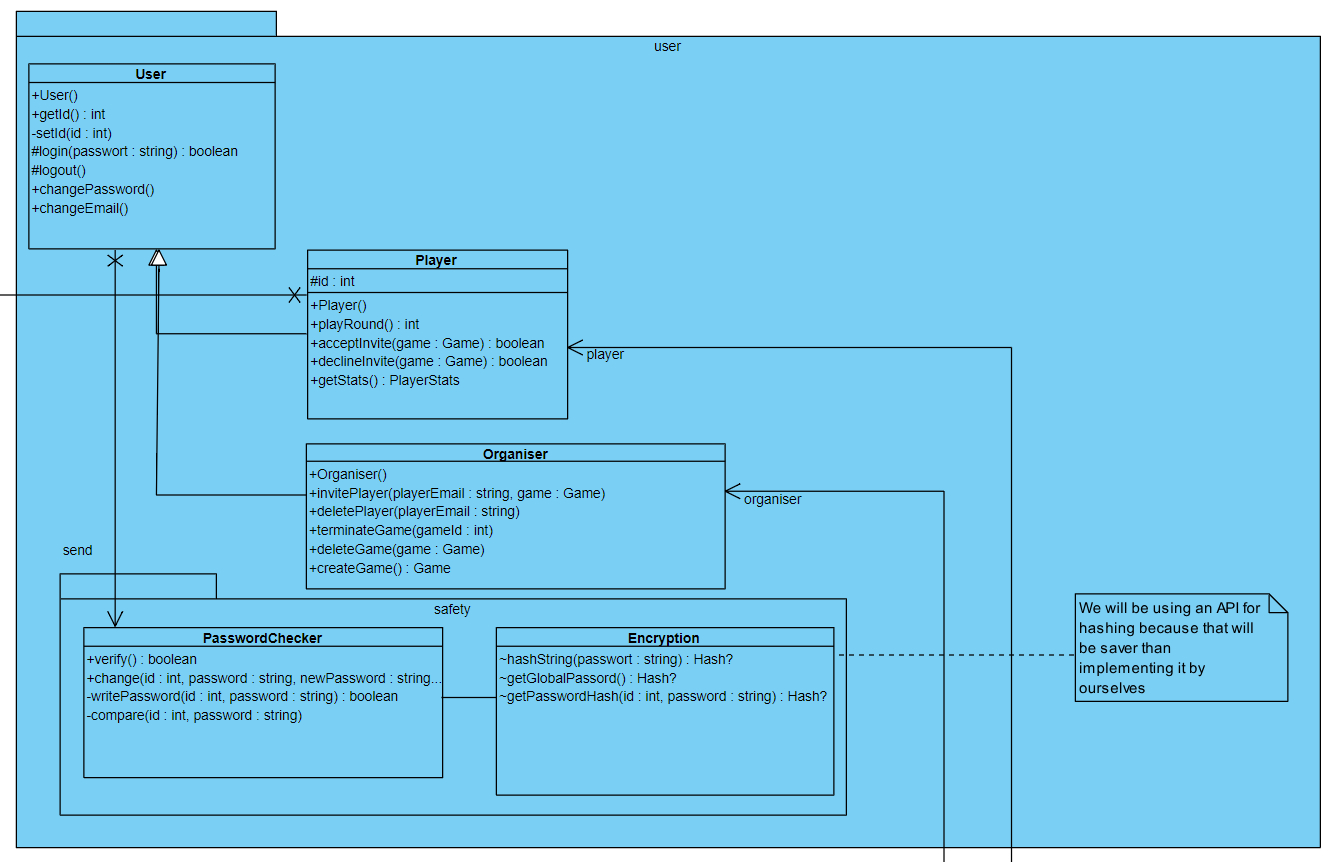
\includegraphics[width=\textwidth]{img/user.png}
	\subsubsection{User}
	Stellt einen Nutzer im System dar.
	\subsubsection{getId}
	\begin{itemize}
		\item Beschreibung: Gibt die eindeutige Id zurück, die einem Nutzer zugeordnet ist
		\item Parameter: int
		\item Rückgabewert: int
	\end{itemize}
	\subsubsection{setId}
	\begin{itemize}
		\item Beschreibung: Diese Methode dient dem Zuordnen einer Id zu einem Spieler. Die Methode überprüft, ob die Id gültig ist (also noch nicht existiert)
		\item Parameter: int
		\item Rückgabewert: void
	\end{itemize}
	\subsubsection{login}
	\begin{itemize}
		\item Beschreibung: Mithilfe dieser Methode loggt sich der Nutzer ein
		\item Parameter: String
		\item Rückgabewert: boolean
	\end{itemize}
	\subsubsection{logout}
	\subsubsection{changePassword}
	\subsubsection{changeEmail}
	
	\subsection{Player}
	\subsection{Organiser}
	
	\section{Safety}
	\subsection{PasswordChecker}
	\subsection{Encryption}
	
	\section{API}
	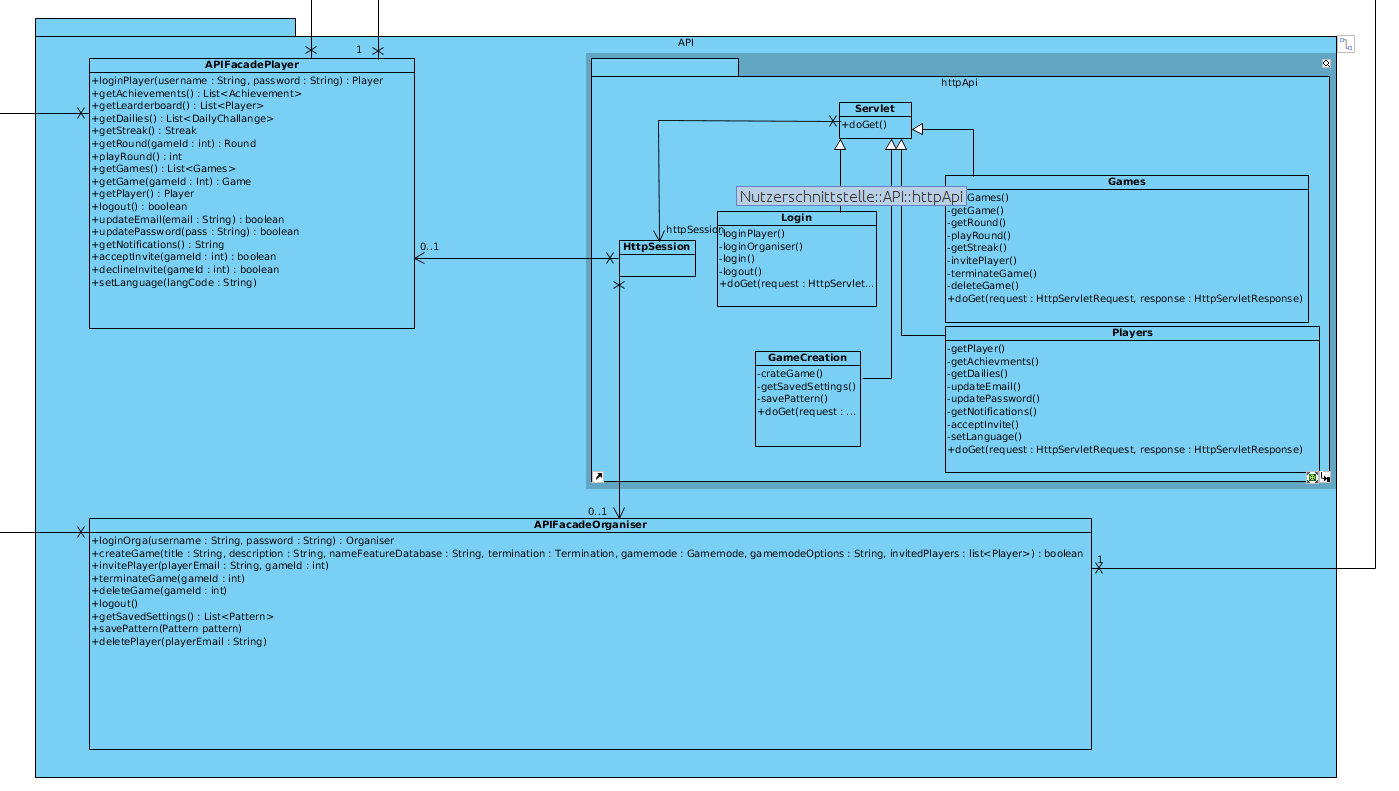
\includegraphics[width=\textwidth]{img/api.png}
	\subsection{APIFacadePlayer}
	Eine APIFacadePlayer ist das Objekt, über welches sämtliche Interaktion mit dem System von den Spielern aus passiert. Nach dem Konstruktor \textbf{muss} zuerst loginPlayer aufgerufen werden, bis es erfolgreich zurückkehrt. Ansonsten haben alle anderen Methoden kein definiertes Verhalten und werden im Allgemeinem nichts nützliches zurückgeben. Eine APIFacadePlayer ist immer mit einem Spieler assoziiert, falls dieser korrekt angemeldet wurde. Alle Methoden beziehen sich dann auf den angemeldeten Spieler.
	\subsubsection{loginPlayer}
	\begin{itemize}
		\item Beschreibung: Versucht einen Spieler mit email und password anzumelden. Bei Erfolg wird diese Fassade mit dem Spieler assoziiert.
		\item Parameters: 
		\begin{itemize}
			\item email: Die E-Mail Adresse, mit der eine Anmeldung versucht wird
			\item password: Das Passwort, mit dem eine Anmeldung versucht wird
		\end{itemize}
		\item Rückgabewert: Falls die E-Mail-Passwort-Kombination einen validen Spieler beschreibt, wird dieser zurückgegeben. Andernfalls wird null zurückgegeben.
	\end{itemize}
	\subsubsection{logout}
	\begin{itemize}
		\item Beschreibung: Meldet den angemeldeten Spieler ab. Nach dem Aufruf dieser Methode verhält sich dieses Objekt wieder so, als ob nie ein Spieler angemeldet wurde
	\end{itemize}
	\subsubsection{getAchievments}
	\begin{itemize}
		\item Beschreibung: Holt die Liste aller Achievments, mit der Information ob der Spieler diese bereits erreicht hat oder nicht.
		\item Rückgabewert: Liste an Achievments. 
	\end{itemize}
	\subsubsection{getLeaderboard}
	\begin{itemize}
		\item Beschreibung: Gibt das aktuelle Leaderboard in der geordneten Reihenfolge zurück
		\item Rückgabewert: Eine Liste an Spielern, geordnet nach ihrer Leaderboard-Ordunung. 
	\end{itemize}
	\subsubsection{getDailies}
	\begin{itemize}
		\item Beschreibung: Gibt die Daily-Challenges für diesen Spieler zurück, mit der Information, ob diese bereits erfüllt sind.
		\item Rückgabewert: Eine Liste an Daily-Challenges für diesen Spieler mit Information, ob diese erfüllt sind.
	\end{itemize}
	\subsubsection{getStreak}
	\begin{itemize}
		\item Beschreibung: Gibt das aktuelle Streak-Objekt für diesen Spieler zurück
		\item Rückgabewert: Das aktuelle Streak-Objekt für diesen Spieler 
	\end{itemize}
	\subsubsection{getPoints}
	\begin{itemize}
		\item Beschreibung: Gibt die Punkte des Spielers zurück
		\item Rückgabewert: Aktuelle Punktzahl des Spielers 
	\end{itemize}
	\subsubsection{getRound}
	\begin{itemize}
		\item Beschreibung: Fordert die nächste Runde für ein Spiel an und gibt diese zurück
		\item Parameter:
		\begin{itemize}
			\item gameId: Eindeutige Id des Spieles für das die Runde angefordert wird
		\end{itemize}
		\item Rückgabewert: Wenn der Spieler eine Runde in dem angegebenem Spiel spielen darf, dann wird das Runden-Objekt zurückgegen. Andernfalls wird null zurückgegeben 
	\end{itemize}
	\subsubsection{playRound}
	\begin{itemize}
		\item Beschreibung: Spielt eine Runde in der aktuellen Runde
	\end{itemize}
	\subsubsection{getGames}
	\begin{itemize}
		\item Beschreibung: Holt alle Spiele, an denen der Spieler teilnimmt
		\item Rückgabewert: Liste an Spielen, an denen der Spieler teilnimmt 
	\end{itemize}
	\subsubsection{getGame}
	\begin{itemize}
		\item Beschreibung: Gibt ein Spiel nach Id zurück, falls der Spieler auf dieses Spiel Zugriff hat
		\item Parameter:
		\begin{itemize}
			\item gameId: die Id des Spiels, welches zurückgegeben werden soll
		\end{itemize}
		\item Rückgabewert: Falls gameId valid ist, also Spiel existiert und Spieler darf auf das Spiel zugreifen, dann wird das Spiel zurückgegen, ansonsten null. 
	\end{itemize}
	\subsubsection{getPlayer}
	\begin{itemize}
		\item Beschreibung: Gibt den angemeldeten Spieler zurück. Also der Spieler, welcher durch loginPlayer angemeldet wurde.
		\item Rückgabewert: Der angemeldete Spieler, falls keiner angemeldet ist wird null zurückgegeben. 
	\end{itemize}
	\subsubsection{updateEmail}
	\begin{itemize}
		\item Beschreibung: Ändert die E-Mail-Adresse mit der sich ein Spieler anmeldet. Die Änderung tritt erst in Effekt, wenn die neue E-Mail-Adresse bestätigt wurde.
		\item Parameter:
		\begin{itemize}
			\item email: Die neue E-Mail-Adresse, welche in Zukunft für diesen Spieler verwendet werden soll.
		\end{itemize}
		\item Rückgabewert: true, falls die Bestätigungsmail veschickt wurde, false andernfalls 
	\end{itemize}
	\subsubsection{updatePassword}
	\begin{itemize}
		\item Beschreibung: Ändert das Passwort, mit dem sich der Spieler anmeldet. Die Änderung tritt sofort in Effekt.
		\item Parameter:
		\begin{itemize}
			\item pass: Das neue Passwort
		\end{itemize}
		\item Rückgabewert: true falls die Änderung erfolgreich war, false andernfalls 
	\end{itemize}
	\subsubsection{getNotifications}
	\begin{itemize}
		\item Beschreibung: Holt alle Notifications, die für diesen Spieler anliegen
		\item Rückgabewert:  Alle Notifications, die für diesen Spieler anliegen
	\end{itemize}
	\subsubsection{acceptInvite}
	\begin{itemize}
		\item Beschreibung: Akzeptiert eine Einladung zu einem Spiel, welche diesem Spieler geschickt wurde und löscht diese aus seinen Einladungen
		\item Parameter:
		\begin{itemize}
			\item gameId: Id des Spiels für das die Einladung angenommen werden soll.
		\end{itemize}
		\item Rückgabewert: true wenn die Einladung angenommen wurde, false falls der Spieler keine Einladung zu diesem Spiel hatte, das Spiel nicht existier oder bereits beendet ist. 
	\end{itemize}
	\subsubsection{declineInvite}
	\begin{itemize}
		\item Beschreibung: Lehnt eine Einladung zu einem Spiel ab, welche diesem Spieler geschickt wurde und löscht diese aus seinen Einladungen
		\item Parameter:
		\begin{itemize}
			\item gameId: Id des Spiels für das die Einladung abgelehnt werden soll.
		\end{itemize}
		\item Rückgabewert: true, wenn die Einladung abgelehnt wurde, false, falls der Spieler keine Einladung zu diesem Spiel hatte, das Spiel nicht existiert oder bereits beendet ist. 
	\end{itemize}
	\subsubsection{setLanguage}
	\begin{itemize}
		\item Beschreibung: Setzt die Sprache für den Spieler
		\item Parameter:
		\begin{itemize}
			\item langCode: der Landescode für die gewünschte Sprache
		\end{itemize}
	\end{itemize}
    \subsubsection{registerPlayer}
    \begin{itemize}
        \item Beschreibung: registriert einen neuen Spieler in das System. Bei diesem Aufruf wird eine E-Mail an die angegebene Email gesendet. Das Passwort muss der Spieler sich merken, da es in den loginPlayer Aufruf benötigt wird.
        \item Parameter:
        \begin{itemize}
            \item email: E-Mail Adresse des zu registrierenden Spielers. Der Spieler muss Zugriff auf diese E-Mail Adresse haben.
            \item password: Das Passwort des neu zu registrierenden Spielers.
            \item username: Der Nutzername des neu zu registrierenden Spielers.
        \end{itemize}
    \end{itemize}
    \subsubsection{validateEmail}
    \begin{itemize}
        \item Beschreibung: Teilt dem System mit, dass die E-Mail Adresse eines Nutzers bestätigt wurde. Optimalerweise durch den Link, welcher in der E-Mail versendet wurde. Kann aber natürlich auf direkt nach dem registerPlayer Aufruf gemacht werden.
    \end{itemize}
	\subsection{APIFacadeOrganiser}
	\subsubsection{loginOrganiser}
	\begin{itemize}
		\item Beschreibung: meldet einen Organisator an. Damit dies möglich ist, muss der Organisator vorher registriert worden sein.
		\item Parameter:
		\begin{itemize}
			\item email: E-Mail des anzumeldenden Organisators
			\item password: Das Passwort des anzumeldenden Organisators
		\end{itemize}
		\item Rückgabewert: Falls die Email-Passwort Kombinnation valid ist, also ein Organisator mit der E-Mail registriert ist und das Passwort ist richtig, wird der Organisator zurückgegeben. Andernfalls null. 
	\end{itemize}
	\subsubsection{createGame}
	\begin{itemize}
		\item Beschreibung: erstellt ein Spiel für diesen Organisator.
		\item Parameter: %% stuff bleibt hier ja noch nicht ganz fest gegeben
		\begin{itemize}
			\item :
		\end{itemize}
		\item Rückgabewert: Falls das Erstellen erfolgreich war, true zurückgegeben, andernfalls false. 
	\end{itemize}
	\subsubsection{invitePlayer}
	\begin{itemize}
		\item Beschreibung: Lädt einen Spieler zu einem Spiel des Organisators ein.
		\item Parameter:
		\begin{itemize}
			\item playerEmail: die Email-Adresse des einzuladenden Spielers
			\item gameId: Das Spiel, zu dem der Spieler eingeladen werden soll. Das Spiel muss ein Spiel des Organisators sein.
		\end{itemize}
	\end{itemize}
	\subsubsection{terminateGame}
	\begin{itemize}
		\item Beschreibung: Beendet ein Spiel des Organisators. 
		\item Parameter:
		\begin{itemize}
			\item gameId: Id des zu beendenden Spiels. Das Spiel muss zu dem Organisator gehören.
		\end{itemize}
	\end{itemize}
	\subsubsection{deleteGame}
	\begin{itemize}
		\item Beschreibung: Löscht ein Spiel des Organisators aus dem System. 
		\item Parameter:
		\begin{itemize}
			\item gameId: Die Id des zu löschenden Spiel
		\end{itemize}
	\end{itemize}
	\subsubsection{logout}
	\begin{itemize}
		\item Beschreibung: Meldet einen Organisator ab. Nach dem Aufruf dieser Methode verhält sich dieses Objekt so, als ob niemand angemeldet war.
	\end{itemize}
	\subsubsection{getSavedSettings}
	\begin{itemize}
		\item Beschreibung: Holt eine Liste aller gespeicherten Einstellungen dieses Organisators.
		\item Rückgabewert: Eine Liste aller gespeichterten Einstellungen dieses Organisators. 
	\end{itemize}
	\subsubsection{savePattern}
	\begin{itemize}
		\item Beschreibung: Speichert eine Einstellungskonfiguration für diesen Organisator
		\item Parameter:
		\begin{itemize}
			\item pattern: Das zu speichernde Pattern
		\end{itemize}
	\end{itemize}
	\subsubsection{registerOrganiser}
    \begin{itemize}
        \item Beschreibung: registriert einen neuen Spieler in das System. Bei diesem Aufruf wird eine E-Mail an die angegebene Email gesendet. Das Passwort muss der Spieler sich merken, da es in den loginOrganiser Aufruf benötigt wird.
        \item Parameter:
        \begin{itemize}
            \item email: E-Mail Adresse des zu registrierenden Organisators. Der Organisator muss Zugriff auf diese E-Mail Adresse haben.
            \item password: Das Passwort des neu zu registrierenden Organisators.
            \item mainPassword: Das Haupt-Passwort, welches in der Konfigurationsdatei steht und benötigt wird um das registrieren als Organisator zu erlauben.
        \end{itemize}
    \end{itemize}
    \subsubsection{validateEmail}
    \begin{itemize}
        \item Beschreibung: Teilt dem System mit, dass die E-Mail Adresse eines Nutzers bestätigt wurde. Optimalerweise durch den Link, welcher in der E-Mail versendet wurde. Kann aber natürlich auf direkt nach dem registerOrganiser Aufruf gemacht werden.
    \end{itemize}
    \subsection{httpAPI}
    Implementierung der beiden Fassadenobjecten für http/REST.

	\begin{comment} Vollständiges Doku-Template
	\begin{itemize}
	\item Beschreibung:
	\item Parameter:
	\item Rückgabewert:
	\end{itemize}
	\end{comment}
	
	\section{Database}
	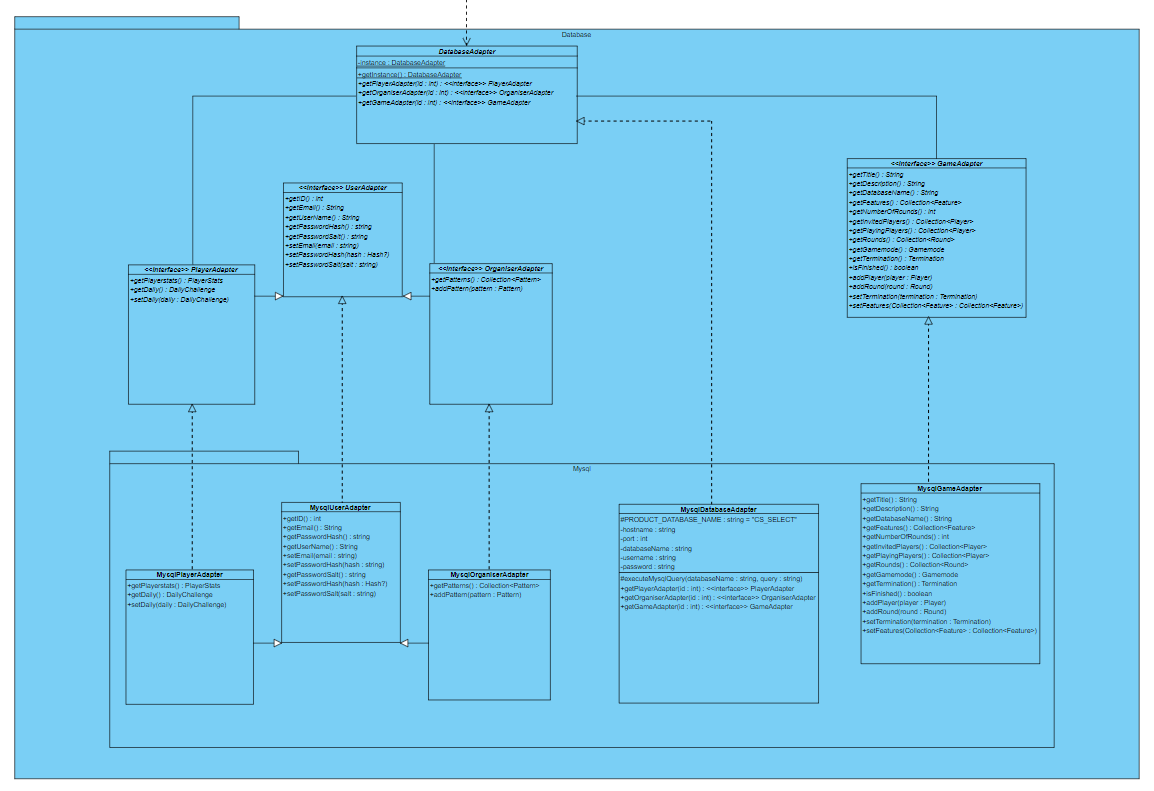
\includegraphics[width=\textwidth]{img/Database.PNG}
	Paket das die Kommunikation mit der Datenbank übernimmt.
	
	\subsection{DatabaseAdapter}
	Abstrakte Klasse die als Singleton realisiert ist und von der jeweiligen Datenbankimplementierung abstrahiert.
	
	\subsubsection{instance}
	Instanz des Singletons die durch Vererbung spezialisiert wird.
	
	\subsubsection{getInstance}
	\begin{itemize}
		\item Beschreibung: Statische Methode, die die Instanz des DatabaseAdapters zurückgibt
		\item Rückgabewert: Instanz des DatabaseAdapters
	\end{itemize}
	
	\subsubsection{getPlayerAdapter}
	\begin{itemize}
		\item Beschreibung: Gibt den PlayerAdapter für den Spieler mit der gegebenen ID zurück.
		\item Parameter:
		\begin{itemize}
			\item id: ID des Spielers, dessen PlayerAdapter zurückgegeben werden soll.
		\end{itemize}
		\item Rückgabewert: PlayerAdapter des Spielers mit ID id.
	\end{itemize}
	
	\subsubsection{getOrganiserAdapter}
	\begin{itemize}
		\item Beschreibung: Gibt den OrganiserAdapter für den Organisator mit der gegebenen ID zurück.
		\item Parameter:
		\begin{itemize}
			\item id: ID des Organisators, dessen OrganiserAdapter zurückgegeben werden soll.
		\end{itemize}
		\item Rückgabewert: OrganiserAdapter des Organisators mit ID id.
	\end{itemize}
	
	\subsubsection{getGameAdapter}
	\begin{itemize}
		\item Beschreibung: Gibt den GameAdapter für das Spiel mit der gegebenen ID zurück.
		\item Parameter:
		\begin{itemize}
			\item id: ID des Spiels, dessen GameAdapter zurückgegeben werden soll.
		\end{itemize}
		\item Rückgabewert: GameAdapter des Spiels mit ID id.
	\end{itemize}

	\subsubsection{getPlayer}
	\begin{itemize}
		\item Beschreibung: Gibt das Player Objekt mit der gegebenen E-Mail-Addresse zurück.
		\item Parameter:
		\begin{itemize}
			\item email: E-Mail-Addresse des Spielers der zurückgegeben werden soll.
		\end{itemize}
		\item Rückgabewert: Player mit der gegebenen E-Mail-Addresse
	\end{itemize}

	\subsubsection{removeGame}
	\begin{itemize}
		\item Beschreibung: Entfernt das gegebene Spiel aus der Datenbank.
		\item Parameter:
		\begin{itemize}
			\item game: Spiel das aus der Datenbank entfernt werden soll.
		\end{itemize}
	\end{itemize}
	
	\subsection{UserAdapter}
	Schnittstelle die Methoden für alle Nutzer des Produkts bereitstellt.
	Jeder UserAdapter ist genau einem Nutzer zugeordnet.
	
	\subsubsection{getID}
	\begin{itemize}
		\item Beschreibung: Gibt die ID des Nutzers zurück.
		\item Rückgabewert: int mit ID des Nutzers.
	\end{itemize}
	
	\subsubsection{getEmail}
	\begin{itemize}
		\item Beschreibung: Gibt die E-Mail-Addresse des Nutzers zurück.
		\item Rückgabewert: String mit E-Mail-Addresse des Nutzers.
	\end{itemize}
	
	\subsubsection{getUsername}
	\begin{itemize}
		\item Beschreibung: Gibt den Nutzernamen des Nutzers zurück.
		\item Rückgabewert: String mit Nutzernamen des Nutzers.
	\end{itemize}
	
	\subsubsection{getPasswordHash}
	\begin{itemize}
		\item Beschreibung: Gibt das gehashte Passwort des Nutzers zurück.
		\item Rückgabewert: Hash des Passworts
	\end{itemize}
	
	\subsubsection{setEmail}
	\begin{itemize}
		\item Beschreibung: Setzt die E-Mail-Adresse des Nutzers neu.
		\item Parameter:
		\begin{itemize}
			\item email: String der neuen E-Mail-Adresse.
		\end{itemize}
	\end{itemize}
	
	\subsubsection{setPassword}
	\begin{itemize}
		\item Beschreibung: Setzt das gehashte Passwort sowie den Salt des Nutzers neu.
		\item Parameter:
		\begin{itemize}
			\item hash: Hash-String des neuen Passworts
			\item salt: Salt-String des neuen Passworts
		\end{itemize}
	\end{itemize}
	
	\subsection{PlayerAdapter}
	Schnittstelle die UserAdapter erweitert.
	Jeder PlayerAdapter ist stets genau einem Spieler zugeordnet.
	
	\subsubsection{getPlayerStats}
	\begin{itemize}
		\item Beschreibung: Gibt die gespeicherten PlayerStats eines Spielers zurück.
		\item Rückgabewert: PlayerStats Objekt des Spielers.
	\end{itemize}
	
	\subsection{OrganiserAdapter}
	Schnittstelle die UserAdapter erweitert.
	Jeder OrganiserAdapter ist stets genau einem Organisator zugeordnet.
	
	\subsubsection{getPatterns}
	\begin{itemize}
		\item Beschreibung: Gibt die gespeicherten Patterns des Organisators zurück.
		\item Rückgabewert: Collection der gespeicherten Patterns des Organisators.
	\end{itemize}
	
	\subsection{GameAdapter}
	Schnittstelle die Methoden für gespeicherte Spiele des Produkts bereitstellt.
	Jeder GameAdapter ist stets genau einem Spiel zugeordnet.
	
	\subsubsection{getTitle}
	\begin{itemize}
		\item Beschreibung: Gibt den Titel des Spiels zurück.
		\item Rückgabewert: String mit Titel.
	\end{itemize}
	
	\subsubsection{getDescription}
	\begin{itemize}
		\item Beschreibung: Gibt die Beschreibung des Spiels zurück.
		\item Rückgabewert: String mit Beschreibung des Spiels.
	\end{itemize}
	
	\subsubsection{getDatabaseName}
	\begin{itemize}
		\item Beschreibung: Gibt den Namen der Datenbank zurück in der das Spiel gespeichert ist.
		\item Rückgabewert: String mit Namen der Datenbank.
	\end{itemize}
	
	\subsubsection{getFeatures}
	\begin{itemize}
		\item Beschreibung: Gibt die Features des Spiels zurück.
		\item Rückgabewert: Collection mit den Features des Spiels.
	\end{itemize}
	
	\subsubsection{getNumberOfRounds}
	\begin{itemize}
		\item Beschreibung: Gibt die Anzahl der zu spielenden Runden zurück.
		\item Rückgabewert: int mit zu spielenden Runden.
	\end{itemize}
	
	\subsubsection{getInvitedPlayers}
	\begin{itemize}
		\item Beschreibung: Gibt die eingeladenen Spieler zurück.
		\item Rückgabewert: Collection mit den eingeladenen Spielern
	\end{itemize}
	
	\subsubsection{getPlayingPlayers}
	\begin{itemize}
		\item Beschreibung: Gibt die spielenden Spieler zurück.
		\item Rückgabewert: Collection mit den spielenden Spielern.
	\end{itemize}
	
	\subsubsection{getRounds}
	\begin{itemize}
		\item Beschreibung: Gibt die gespielten Runden zurück.
		\item Rückgabewert: Collection der gespielten Runden.
	\end{itemize}
	
	\subsubsection{getGamemode}
	\begin{itemize}
		\item Beschreibung: Gibt den gewählten Spielmodus zurück.
		\item Rückgabewert: Gamemode
	\end{itemize}
	
	\subsubsection{getTermination}
	\begin{itemize}
		\item Beschreibung: Gibt die Art der Spielterminierung zurück.
		\item Rückgabewert: Termination
	\end{itemize}
	
	\subsubsection{isFinished}
	\begin{itemize}
		\item Beschreibung: Gibt zurück ob das Spiel beendet wurde oder nicht.
		\item Rückgabewert: True falls das Spiel beendet wurde, false sonst
	\end{itemize}
	
	\subsubsection{addPlayer}
	\begin{itemize}
		\item Beschreibung: Fügt einen Spieler zum Spiel hinzu.
		\item Parameter:
		\begin{itemize}
			\item player: Spieler der hinzugefügt werden soll.
		\end{itemize}
	\end{itemize}
	
	\subsubsection{addRound}
	\begin{itemize}
		\item Beschreibung: Fügt eine Runde zum Spiel hinzu.
		\item Parameter:
		\begin{itemize}
			\item round: Runde die hinzugefügt werden soll.
		\end{itemize}
	\end{itemize}
	
	\subsubsection{setTermination}
	\begin{itemize}
		\item Beschreibung: Setzt die Art der Spielterminierung.
		\item Parameter:
		\begin{itemize}
			\item termination: Termination Objekt das die Art der Spielterminierung festlegt.
		\end{itemize}
	\end{itemize}
	
	\subsubsection{setFeatures}
	\begin{itemize}
		\item Beschreibung: Setzt die Features des Spiels.
		\item Parameter:
		\begin{itemize}
			\item features: Collection mit den Features des Spiels.
		\end{itemize}
	\end{itemize}

	\subsubsection{setFinished}
	\begin{itemize}
		\item Beschreibung: Setzt das Spiel auf beendet.
	\end{itemize}
	
	\subsection{Mysql}
	Paket mit Mysql basierter Implementierung der Datenbank.
	Mitgelieferte Standard-Implementierung des Produkts.
	
	\subsubsection{MysqlDatabaseAdapter}
	Mysql Implementierung der DatabaseAdapter Klasse.

	\paragraph{executeMysqlQuery}
	\begin{itemize}
		\item Beschreibung: Führt den gegebenen Mysql Query auf der Datenbank mit dem gegebenen Namen aus.
		\item Parameter:
		\begin{itemize}
			\item databaseName: Name der zu nutzenden Datenbank
			\item query: Auszuführender Mysql-Query
		\end{itemize}
	\end{itemize}
	
	\subsubsection{MysqlUserAdapter}
	Mysql Implementierung der UserAdapter Schnittstelle.
	
	\subsubsection{MysqlPlayerAdapter}
	Mysql Implementierung der PlayerAdapter Schnittstelle.
	Erbt von MysqlUserAdapter
	
	\subsubsection{MysqlOrganiserAdapter}
	Mysql Implementierung der OrganiserAdapter Schnittstelle.
	Erbt von MysqlUserAdapter
	
	\subsubsection{MysqlGameAdapter}
	Mysql Implementierung der GameAdapter Schnittstelle.
	
	\section{Configuration}
	Paket für die Kommunikation mit der Konfigurationsdatei.
	
	\subsection{Configuration}
	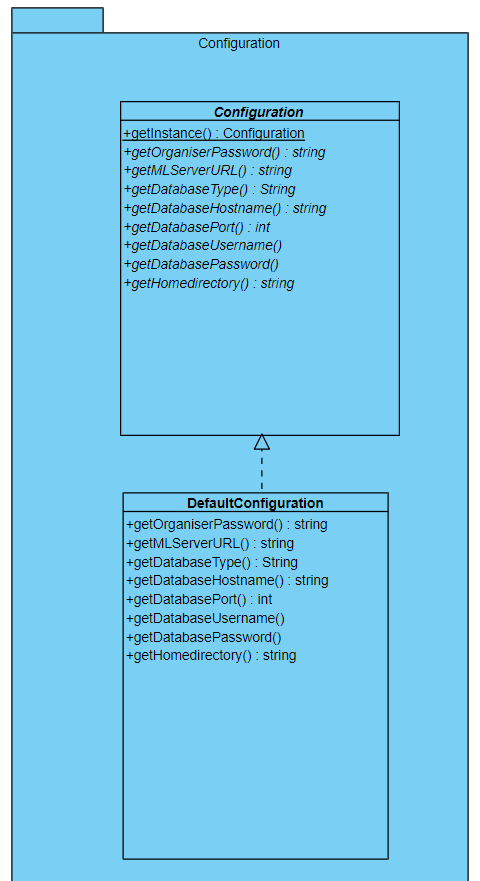
\includegraphics[width=\textwidth]{img/Configuration.PNG}
	Abstrakte Klasse die von der Config-Implementierung abstrahiert.
	Kümmert sich um die Kommunikation des Produkts mit der Konfigurationsdatei.
	Ist als Singleton umgesetzt um zu erzwingen, dass stets nur ein Zugriffspunkt zur Konfiguration besteht.
	
	\subsubsection{getInstance}
	\begin{itemize}
		\item Beschreibung: Statische Methode die die Instanz der Configuration zurückgibt.
		\item Rückgabewert: Instanz der Configuration.
	\end{itemize}
	
	
	\subsubsection{getOrganiserPassword}
	\begin{itemize}
		\item Beschreibung: Gibt das Passwort als String zurück das Organisatoren bei der Erstregistrierung verwenden müssen.
		\item Rückgabewert: String mit Organisatorpasswort
	\end{itemize}
	
	\subsubsection{getMLServerURL}
	\begin{itemize}
		\item Beschreibung: Gibt die URL als String zurück, unter der der ML-Server zu finden ist
		\item Rückgabewert: String mit URL des ML-Servers
	\end{itemize}
	
	\subsubsection{getDatabaseType}
	\begin{itemize}
		\item Beschreibung: Gibt die Art der verwendeten Datenbankimplementierung zurück.
		\item Rückgabewert: String mit Name der Datenbankimplementierung.
	\end{itemize}
	
	\subsubsection{getDatabaseHostname}
	\begin{itemize}
		\item Beschreibung: Gibt den Hostnamen des Datenbankservers zurück.
		\item Rückgabewert: String mit Hostnamen des Datenbankservers.
	\end{itemize}
	
	\subsubsection{getDatabasePort}
	\begin{itemize}
		\item Beschreibung: Gibt den Port des Datenbankservers zurück.
		\item Rückgabewert: int mit Port des Datenbankservers.
	\end{itemize}
	
	\subsubsection{getDatabaseUsername}
	\begin{itemize}
		\item Beschreibung: Gibt den Nutzernamen mit dem sich am Datenbankserver angemeldet wird zurück.
		\item Rückgabewert: String mit Nutzernamen
	\end{itemize}
	
	\subsubsection{getDatabasePassword}
	\begin{itemize}
		\item Beschreibung: Gibt das Passwort mit dem sich am Datenbankserver angemeldet wird zurück.
		\item Rückgabewert: String mit Passwort
	\end{itemize}
	
	\subsection{DefaultConfiguration}
	Implementiert die abstrakte Klasse Configuration und stellt die Funktionalität bereit.
	Mitgelieferte Standardimplementierung der Konfiguration.
	
	\section{MLServer}
	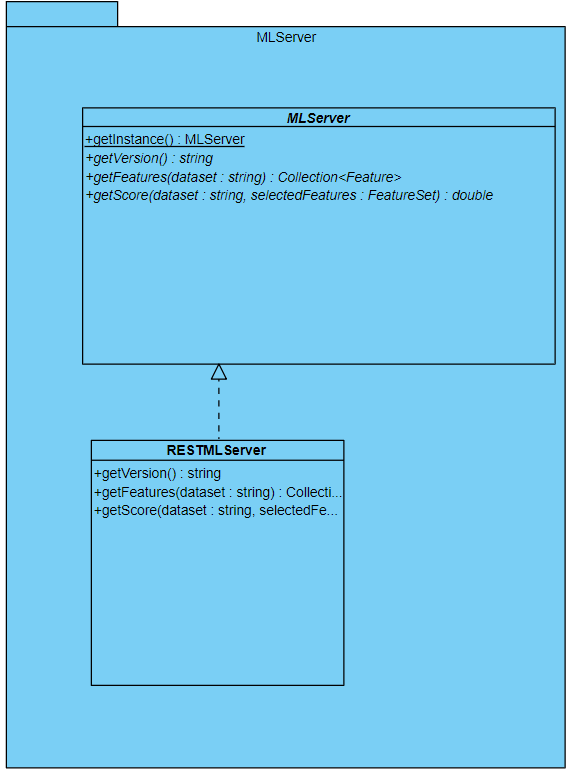
\includegraphics[width=\textwidth]{img/MLServer.PNG}
	Paket für die Kommunikation mit dem ML-Server.
	
	\subsection{MLServer}
	Abstrakte Klasse die von der Implementierung der ML-Server-API abstrahiert.
	Ist als Singleton umgesetzt um zu erzwingen dass stets nur ein Zugriffspunkt zum ML-Server existiert.
	
	\subsubsection{getInstance}
	\begin{itemize}
		\item Beschreibung: Statische Methode die die Instanz des MLServers zurückgibt.
		\item Rückgabewert: Instanz des MLServers.
	\end{itemize}
	
	\subsubsection{getVersion}
	\begin{itemize}
		\item Beschreibung: Gibt die Version des genutzten ML-Servers als String zurück.
		\item Rückgabewert: String mit der Versionsnummer.
	\end{itemize}
	
	\subsubsection{getFeatures}
	\begin{itemize}
		\item Beschreibung: Gibt die Features des angegebenen Datensatzes zurück
		\item Parameter:
		\begin{itemize}
			\item dataset: Datensatz dessen Features zurückgegeben werden sollen.
		\end{itemize}
		\item Rückgabewert: Collection mit den Features des Datensatzes.
	\end{itemize}
	
	\subsubsection{getScore}
	\begin{itemize}
		\item Beschreibung: Gibt die Bewertung der gesendeten Features zurück.
		\item Parameter:
		\begin{itemize}
			\item dataset: Datensatz von dem eine Merkmalsauswahl geschickt wird.
			\item selectedFeatures: Ausgewählte Merkmale.
		\end{itemize}
		\item Rückgabewert: double mit Wert im Intervall [0,1] der die Güte der Auswahl beschreibt.
	\end{itemize}
	
	\subsection{RESTMLServer}
	Implementiert die abstrakte Klasse MLServer und stellt die Funktionalität mittels der Standard-Implementierung des ML-Servers per REST-API bereit.
	
	
	
	
	
	
	
	
	
	
	
	
	\section{Game}
	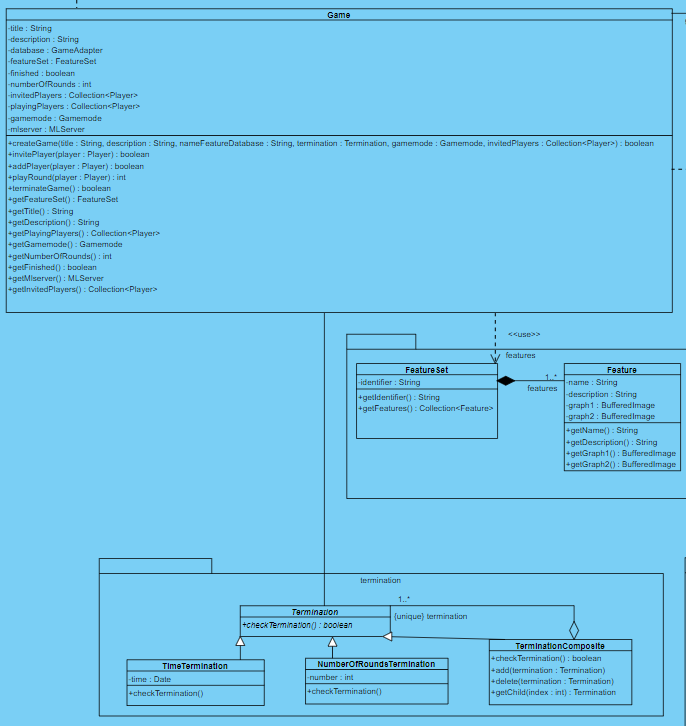
\includegraphics[width=\textwidth]{img/GameTerminationFeature.PNG}
	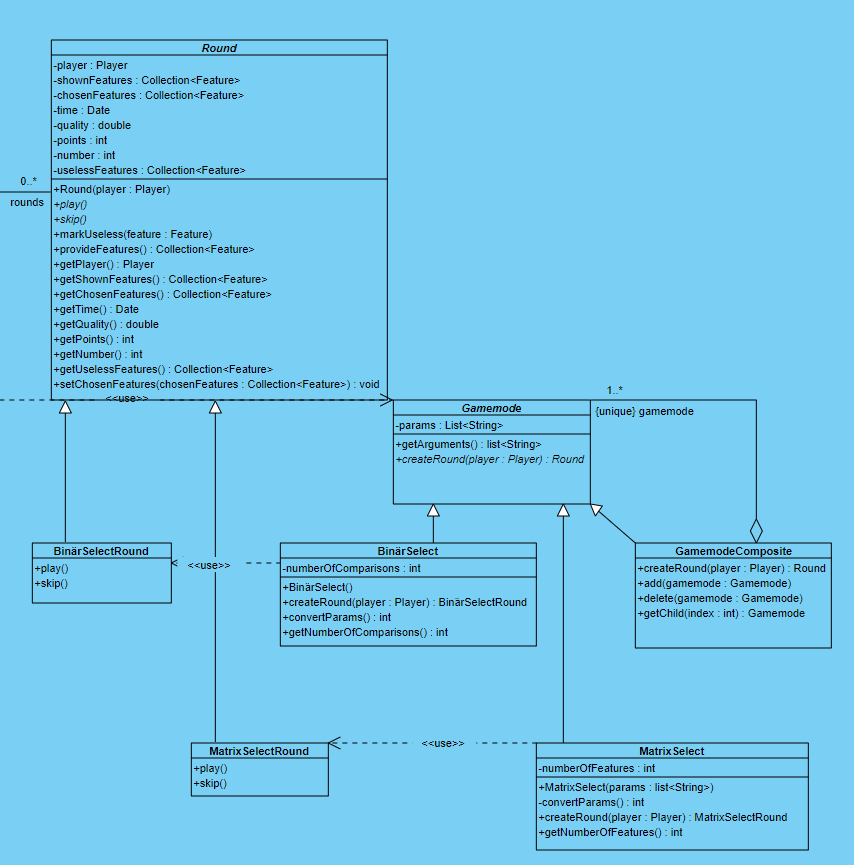
\includegraphics[width=\textwidth]{img/RoundAndGameMode.PNG}
	Paket, welches die innere Spielmechanik verwaltet. Dazu gehören die Spiele mit ihrer Erstellung und ihren Abbruchbedingungen, Spielmodi, Runden und Merkmale.
	
	\subsection{Game}
	Stellt ein Spiel dar, verwaltet eingeladene und spielende Spieler sowie die zum Spiel zugehörigen Informationen
	\subsubsection{Game}
	\begin{itemize}
	\item Beschreibung: Konstruktor, der ein Game-Objekt erzeugt, die ID wird auf die nächst freie ID gesetzt und der statische Zähler hochgezählt, finished wird auf false gesetzt, numberOfRounds auf 0	
	\end{itemize}
	
	\subsubsection{getTitle}
	\begin{itemize}
		\item Beschreibung: Gibt den Spieltitel zurück
		\item Rückgabewert: Der Spieltitel
	\end{itemize}
	\subsubsection{getDescription}
	\begin{itemize}
		\item Beschreibung: Gibt die Spielbeschreibung zurück
		\item Rückgabewert: Die Spielbeschreibung
	\end{itemize}
	\subsubsection{getFinished}
			\begin{itemize}
				\item Beschreibung: Gibt zurück, ob das Spiel noch aktiv ist
				\item Rückgabewert: False, falls Spiel beendet wurde, sonst true
			\end{itemize}
	\subsubsection{getNumberOfRounds}
		\begin{itemize}
			\item Beschreibung: Gibt die Anzahl der bereits gespielten Runden insgesamt zurück
			\item Rückgabewert: Die Anzahl der gespielten Runden
		\end{itemize}
	\subsubsection{getID}
		\begin{itemize}
		\item Beschreibung: Gibt die ID des Spiels zurück
		\item Rückgabewert: Die ID
		\end{itemize}     
	\subsubsection{getInvitedPlayers}
		\begin{itemize}
			\item Beschreibung: Gibt eine Aufzählung aller Spieler zurück, die eingeladen sind, die Einladung aber noch nicht angenommen haben
			\item Rückgabewert: Die Aufzählung der eingeladenen Spieler
		\end{itemize}
	\subsubsection{getPlayingPlayers}
		\begin{itemize}
			\item Beschreibung: Gibt eine Aufzählung aller Spieler zurück, die die Einladung angenommen haben und Runden spielen können
			\item Rückgabewert: Die Aufzählung der spielenden Spieler
		\end{itemize}
	\subsubsection{getDatabase}
	\begin{itemize}
	\item Beschreibung: Gibt die zum Spiel gehörige Datenbank zurück
	\item Rückgabewert: Die zum Spiel gehörige Datenbank
	\end{itemize}
	\subsubsection{getTermination}
	\begin{itemize}
		\item Beschreibung: Gibt die zum Spiel gehörige Abbruchbedingung zurück
		\item Rückgabewert: Die zum Spiel gehörige Abbruchbedingung
		\end{itemize}
	\subsubsection{getFeatureSet}
		\begin{itemize}
			\item Beschreibung: Gibt den zum Spiel gehörigen Merkmalsdatensatz zurück
			\item Rückgabewert: Der Merkmalsdatensatz
		\end{itemize}	
	\subsubsection{getGamemode}
	\begin{itemize}
		\item Beschreibung: Gibt den zum Spiel gehörigen Spielmodus zurück
		\item Rückgabewert: Der Spielmodus
	\end{itemize}
	\subsubsection{getMlserver}
	\begin{itemize}
		\item Beschreibung: Gibt den ML-Server an, der die Merkmale bereitstellt und die Qualitätsberechnung durchführt
		\item Rückgabewert: Der ML-Server
	\end{itemize}
	\subsubsection{getRounds}
	\begin{itemize}
		\item Beschreibung: Gibt die bisher abgeschlossenen, zum Spiel gehörigen Runden zurück
		\item Rückgabewert: Die abgeschlossenen Runden
		\end{itemize}
	\subsubsection{setTitle}
		\begin{itemize}
		\item Beschreibung: Setzt den Spieltitel auf den angegebenen Wert
		\item Parameter: title: Der Spieltitel
		\end{itemize}
	\subsubsection{setDescription}
		\begin{itemize}
		\item Beschreibung: Setzt die Spielbeschreibung auf den angegebenen Wert
		\item Parameter: description: Die Spielbeschreibung
		\end{itemize}
	\subsubsection{setDatabase}
		\begin{itemize}
		\item Beschreibung: Speichert die angegebene Datenbank als die zum Spiel gehörige
		\item Parameter: database: Die Datenbank, in die die Spielinformationen geschrieben werden
		\end{itemize}
	\subsubsection{setTermination}
		\begin{itemize}
		\item Beschreibung: Setzt die Abbruchbedingung, die bestimmt, wann das Spiel terminiert
		\item Parameter: termination: Die Abbruchbedingung des Spiels
		\end{itemize}
	\subsubsection{setGamemode}
		\begin{itemize}
		\item Beschreibung: Setzt den Spielmodus des Spiels auf den angegebenen Spielmodus
		\item Parameter: gamemode: Der Spielmodus des Spiels
		\end{itemize}
	\subsubsection{setFeatureSet}
		\begin{itemize}
		\item Beschreibung: Speichert den angegebenen Merkmalsdatensatz als den zum Spiel gehörigen
		\item Parameter: featureset: Der Merkmalsdatensatz, aus dem die im Spiel angezeigten Merkmale kommen
		\end{itemize}
	\subsubsection{setMlserver}
		\begin{itemize}
		\item Beschreibung: Speichert den angegebenen ML-Server als den zum Spiel gehörigen
		\item Parameter: mlserver: Der ML-Server, von dem der Merkmalsdatensatz kommt und der die Bewertung durchführt
		\end{itemize}
	\subsubsection{invitePlayer}
		\begin{itemize}
			\item Beschreibung: Fügt dem Spiel Spieler hinzu, die eingeladen wurden
			\item Parameter: players: Die eingeladenen Spieler
			\item Rückgabewert: Ob Spieler erfolgreich hinzugefügt wurden oder schon im Spiel vorhanden sind
		\end{itemize}
	\subsubsection{acceptInvite}
		\begin{itemize}
			\item Beschreibung: Gibt einem Spieler die Spielberechtigung, der eine Einladung erhalten und diese angenommen hat
			\item Parameter: playerID: ID des Spielers, der die Einladung angenommen hat
			\item Rückgabewert: Ob Spieler erfolgreich hinzugefügt wurde oder entweder schon spielt oder keine Einladung hatte
		\end{itemize}
	\subsubsection{declineInvite}
		\begin{itemize}
			\item Beschreibung: Löscht einen Spieler aus den eingeladenen Spielern, der eine Einladung abgelehnt hat
			\item Parameter: playerID: ID des Spielers, der die Einladung abgelehnt hat
			\item Rückgabewert: False, falls der Spieler gar keine aktive Einladung hatte
		\end{itemize}
	\subsubsection{deletePlayer}
		\begin{itemize}
			\item Beschreibung: Löscht einen Spieler aus dem Spiel, sowohl falls er nur eingeladen ist als auch falls er schon spielt
			\item Parameter: playerID: ID des Spielers, der gelöscht werden soll
			\item Rückgabewert: False, falls der Spieler dem Spiel nicht bekannt ist
		\end{itemize}
	\subsubsection{startRound}
		\begin{itemize}
			\item Beschreibung: Startet das Spielen einer Runde durch einen Spieler, erzeugt dafür ein Rundenobjekt, auf dem es die start-Methode aufruft und die anzuzeigenden Merkmale zurückbekommt und selbst zurückgibt
			\item Parameter: playerID: ID des Spielers, der die Runde spielt
			\item Rückgabewert: Die Merkmale, die dem Spieler insgesamt anzuzeigen sind
		\end{itemize}
	\subsubsection{terminateGame}
		\begin{itemize}
			\item Beschreibung: Beendet ein Spiel
			\item Rückgabewert: Ob das Spiel erfolgreich beendet wurde
		\end{itemize}
	\subsubsection{addFinishedRound}
	\begin{itemize}
	\item Beschreibung: Fügt eine Runde zu den abgeschlossenen Runden hinzu
	\item Parameter: round: Die abgeschlossene Runde
	\end{itemize}
	
	\subsection{FeatureSet}
	Stellt einen Merkmalsdatensatz dar, der aus beliebig vielen, aber mindestens einem Merkmal besteht und ohne diese keine Daseinsberechtigung hat
	\subsubsection{FeatureSet}
		\begin{itemize}
		\item Beschreibung: Konstruktor, der ein FeatureSet-Objekt erzeugt
		\item Parameter: identifier: Der Identifikationsschlüssel des Merkmalsdatensatzes
		\end{itemize}
	\subsubsection{getIdentifier}
	\begin{itemize}
		\item Beschreibung: Gibt den eindeutigen Identifikationsschlüssel eines Merkmalsdatensatzes zurück
		\item Rückgabewert: Der Identifikationsschlüssel
	\end{itemize}
	\subsubsection{getFeatures}
	\begin{itemize}
		\item Beschreibung: Gibt die zum Merkmalsdatensatz gehörigen Merkmale zurück
		\item Rückgabewert: Aufzählung der Merkmale
	\end{itemize}
	\subsubsection{addFeature}
	\begin{itemize}
	\item Beschreibung: Fügt ein Merkmal zum Merkmalsdatensatz hinzu
	\item Parameter: feature: Das Merkmal, das hinzugefügt werden soll	
	\subsection{Feature}
	Stellt ein zu einem Merkmalsdatensatz gehöriges Merkmal dar
	\subsubsection{Feature}
		\begin{itemize}
		\item Beschreibung: Konstruktor, der ein Feature-Objekt erzeugt
		\item Parameter: 
		\begin{itemize}
		\item name: Der Name des Merkmals
		\item description: Die Beschreibung des Merkmals
		\item totalGraph: Der Graph des Merkmals, der die Daten insgesamt anzeigt
		\item classGraph: Der  Graph des Merkmals, der die Daten nach Klassen aufgeteilt anzeigt
		\end{itemize}	
		\end{itemize}
	\subsubsection{getName}
	\begin{itemize}
		\item Beschreibung: Gibt den Namen des Merkmals zurück
		\item Rückgabewert: Der Name
	\end{itemize}
	\subsubsection{getDescription}
	\begin{itemize}
		\item Beschreibung: Gibt die Beschreibung des Merkmals zurück
		\item Rückgabewert: Die Beschreibung
	\end{itemize}
	\subsubsection{getTotalGraph}
	\begin{itemize}
		\item Beschreibung: Gibt den Graphen des Merkmals zurück, der die Daten insgesamt anzeigt
		\item Rückgabewert: Der Graph mit Gesamtdaten
	\end{itemize}
	\subsubsection{getClassGraph}
	\begin{itemize}
		\item Beschreibung: Gibt den Graphen des Merkmals zurück, der die Daten nach Klassen aufgeteilt anzeigt
		\item Rückgabewert: Der Graph mit den Klassendaten
	\end{itemize}
	
	\subsection{Termination}
	Stellt eine Abbruchbedingung, die zu einem Spiel gehört, dar
	\subsubsection{checkTermination}
	\begin{itemize}
		\item Beschreibung: Überprüft, ob die Abbruchbedingung erfüllt ist und beendet gegebenenfalls das Spiel
		\item Rückgabewert: True, wenn Bedinung erfüllt war, false sonst
	\end{itemize}
	
	\subsection{TerminationComposite}
	Stellt ein Kompositum aus eindeutigen Abbruchbedingungen dar, um unterschiedliche Abbruchbedingungen für ein Spiel zuzulassen, eine spezielle Abbruchbedingung
	\subsubsection{TerminationComposite}
		\begin{itemize}
		\item Beschreibung: Konstruktor, der ein TerminationComposite-Objekt erzeugt	
		\end{itemize}
	\subsubsection{checkTermination}
	\begin{itemize}
		\item Beschreibung: Implementiert checkTermination von Termination, in dem für jede zugehörige Abbruchbedingung diese Methode ausgeführt wird
	\end{itemize}
	\subsubsection{add}
	\begin{itemize}
		\item Beschreibung: Fügt eine Abbruchbedingung zum Kompositum hinzu
		\item Parameter: termination: die Abbruchbedingung
	\end{itemize}
	\subsubsection{delete}
	\begin{itemize}
		\item Beschreibung: Entfernt eine Abbruchbedingung aus dem Kompositum
		\item Parameter: termination: die zu entfernende Abbruchbedingung
	\end{itemize}
	
	
	\subsection{TimeTermination}
	Sorgt dafür, dass ein Spiel zu einer bestimmten Zeit terminiert
	\subsubsection{TimeTermination}
		\begin{itemize}
		\item Beschreibung: Konstruktor, der ein TimeTermination-Objekt erzeugt
		\item Parameter: time: Die Zeit, zu der das Spiel terminieren soll	
		\end{itemize}
	\subsubsection{checkTermination}
	\begin{itemize}
		\item Beschreibung: Implementiert die Methode, in dem überprüft wird, ob die Zeit erreicht ist
	\end{itemize}
	
	\subsection{NumberOfRoundsTermination}
	Sorgt dafür, dass ein Spiel nach bestimmter Anzahl an gespielten Runden terminiert
	\subsubsection{NumberOfRoundsTermination}
		\begin{itemize}
		\item Beschreibung: Konstruktor, der ein NumberOfRoundsTermination-Objekt erzeugt
		\item Parameter: number: Die Anzahl an Runden, nach der das Spiel terminieren soll	
		\end{itemize}
	\subsubsection{checkTermination}
	\begin{itemize}
		\item Beschreibung: Implementiert die Methode, in dem geprüft wird, ob die Rundenzahl erreicht ist
	\end{itemize}
	
	\subsection{Round}
	Stellt eine konkrete Runde eines bestimmten Spiels dar
	\subsubsection{Round}
		\begin{itemize}
		\item Beschreibung: Konstruktor, der ein Round-Objekt erzeugt
		\item Parameter: 
		\begin{itemize}
		\item player: Der Spieler, der die Runde spielt
		\item number: Die Zahl gibt an, die wievielte Runde des Spiels diese Runde ist
		\end{itemize}
		\end{itemize}
	\subsubsection{getShownFeatures}
	\begin{itemize}
		\item Beschreibung: Gibt die Merkmale zurück, die dem Spieler angezeigt werden
		\item Rückgabewert: Die angezeigten Merkmale
	\end{itemize}
	\subsubsection{getChosenFeatures}
	\begin{itemize}
		\item Beschreibung: Gibt die Merkmale zurück, die vom Spieler ausgewählt wurden
		\item Rückgabewert: Die ausgewählten Merkmale
	\end{itemize}
	\subsubsection{getTime}
	\begin{itemize}
		\item Beschreibung: Gibt den Zeitpunkt zurück, an dem die Runde gestartet wurde
		\item Rückgabewert: Der Startzeitpunkt 
	\end{itemize}
	\subsubsection{getQuality}
	\begin{itemize}
		\item Beschreibung: Gibt die Bewertung der Merkmalsauswahl durch den ML-Server zurück
		\item Rückgabewert: Die Bewertung zwischen 0 und 1
	\end{itemize}
	\subsubsection{getPoints}
	\begin{itemize}
		\item Beschreibung: Gibt die Anzahl an Punkten zurück, die der Spieler durch die Runde dazubekommen hat
		\item Rückgabewert: Die Anzahl der Punkte der Runde
	\end{itemize}
	\subsubsection{getNumberOfRound}
	\begin{itemize}
		\item Beschreibung: Gibt zurück, die wievielte Runde des Spiels diese Runde war
		\item Rückgabewert: Die Nummer der Runde
	\end{itemize}
	\subsubsection{getUselessFeatures}
	\begin{itemize}
		\item Beschreibung: Gibt alle Merkmale zurück, die als unwichtig markiert wurden
		\item Rückgabewert: Die unwichtigen Merkmale
	\end{itemize}
	\subsubsection{getPlayer}
		\begin{itemize}
			\item Beschreibung: Gibt den Spieler zurück, der die Runde spielt
			\item Rückgabewert: Der Spieler
		\end{itemize}
	\subsubsection{start}
		\begin{itemize}
			\item Beschreibung: Abstrakt, startet Runde aus, stellt Merkmale für die GUI bereit und gibt diese zurück
			\item Rückgabewert: Alle Merkmale, die dem Spieler insgesamt in dieser Runde angezeigt werden sollen
		\end{itemize}
	\subsubsection{skip}
		\begin{itemize}
			\item Beschreibung: Abstrakt, beendet die aktuelle Merkmalsauswahl ohne Auswahl durch den Spieler
		\end{itemize}	
	\subsubsection{manageFeatureSelection}
	\begin{itemize}
	\item Beschreibung: Nimmt die Auswahl des Spielers entgegen, lässt die Qualität durch den ML-Server und die Punktzahl durch das zum Spieler gehörigen Gamification-Objekt berechnen und sorgt dafür, dass die Runde in die Datenbank und das Spiel geschrieben wird, gibt die Punktzahl zurück
	\item Parameter: selectedFeatures: Die vom Spieler ausgewählten Merkmale
	\item Rückgabewert: Die mit der Merkmalsauswahl erreichte Punkzahl der Runde
	\end{itemize}
	\subsubsection{hashCode}
	\begin{itemize}
	\item Beschreibung: Abstrakt, berechnet für das Rundenobjekt einen eindeutigen Hashcode
	\item Rückgabewert: Der Hashcode als integer
	\end{itemize}
	\subsubsection{provideFeatures}
				\begin{itemize}
					\item Beschreibung: Abstrakt, wählt Merkmale aus dem zum Spiel gehörigen Merkmalen aus, die dem Spieler angezeigt werden sollen
					\item Rückgabewert: Die Aufzählung der Merkmale
				\end{itemize}
	\subsubsection{markUseless}
		\begin{itemize}
			\item Beschreibung: Fügt Merkmale zu den unwichtigen Merkmalen hinzu
			\item Parameter: features: Die unwichtigen Merkmale
		\end{itemize}
	
	\subsection{StandardRound}
	Fasst alle Runden zusammen, die sich nur anhand der Zahl ihrer Vergleiche, der angezeigten Merkmale oder der auszuwählenden Merkmale unterscheiden
	\subsubsection{getNumberOfComparisons}
	\begin{itemize}
		\item Beschreibung: Gibt die Anzahl an Vergleichen pro Runde zurück
		\item Rückgabewert: Anzahl an Vergleichen
	\end{itemize}
	\subsubsection{getFeaturesPerComparison}
	\begin{itemize}
		\item Beschreibung: Gibt die Anzahl an Merkmalen zurück, die pro Vergleich angezeigt werden
		\item Rückgabewert: Anzahl an Merkmalen pro Vergleich
	\end{itemize}
	\subsubsection{getMinSelect}
	\begin{itemize}
		\item Beschreibung: Gibt die Anzahl an Merkmalen zurück, die pro Vergleich minimal ausgewählt werden müssen
		\item Rückgabewert: Die Anzahl an Merkmalen
	\end{itemize}
	\subsubsection{getMaxSelect}
	\begin{itemize}
		\item Beschreibung: Gibt die Anzahl an Merkmalen zurück, die pro Vergleich maximal ausgewählt werden müssen
		\item Rückgabewert: Die Anzahl an Merkmalen
	\end{itemize}
	\subsubsection{provideFeatures}
	\begin{itemize}
	\item Beschreibung: Wählt pro Vergleich die angegebene Anzahl an Merkmalen aus und gibt diese alle in einer Liste hintereinander zurück
	\end{itemize}
		
	\subsection{BinärSelectRound}
	Eine Runde des Spielmodus BinärSelect, eine Spezialisierung einer Standard-Runde mit 5 Vergleichen von je 2 Merkmalen, von denen eins ausgewählt werden muss
	\subsubsection{BinärSelectRound}
		\begin{itemize}
		\item Beschreibung: Konstruktor, der ein BinärSelectRound-Objekt erzeugt
		\item Parameter:
		\begin{itemize}
				\item player: Der Spieler, der die Runde spielt
				\item number: Die Zahl gibt an, die wievielte Runde des Spiels diese Runde ist
				\end{itemize}
		\end{itemize}
	\subsubsection{start}
	\begin{itemize}
		\item Beschreibung: Sorgt für das Starten der Runde nach den Regeln des Spielmodus BinärSelect
	\end{itemize}
	\subsubsection{skip}
	\begin{itemize}
		\item Beschreibung: Sorgt für das Überspringen eines Vergleiches nach den Regeln des Spielmodus BinärSelect
	\end{itemize}
	\subsubsection{hashCode}
	\begin{itemize}
	\item Beschreibung: Berechnet den Hashcode und gibt ihn als Integer zurück
	\end{itemize}
	
	\subsection{MatrixSelectRound}
	Eine Runde des Spielmodus MatrixSelect, eine Spezialisierung einer Standard-Runde mit einem Vergleich
	\subsubsection{MatrixSelectRound}
		\begin{itemize}
		\item Beschreibung: Konstruktor, der ein MatrixSelectRound-Objekt erzeugt
		\item Parameter: 
		\begin{itemize}
				\item numberOfFeatures: Die Anzahl an Merkmalen, die pro Runde angezeigt werden müssen
				\item minSelect: Die Anzahl an Merkmalen, die pro Runde mindestens ausgewählt werden müssen
				\item maxSelect: Die Anzahl an Merkmalen, die pro Runde maximal ausgewählt werden müssen
				\item player: Der Spieler, der die Runde spielt
				\item number: Die Zahl gibt an, die wievielte Runde des Spiels diese Runde ist
				\end{itemize}	
		\end{itemize}
	\subsubsection{start}
	\begin{itemize}
		\item Beschreibung: Sorgt für das Starten der Runde nach den Regeln des Spielmodus MatrixSelect
	\end{itemize}
	\subsubsection{skip}
	\begin{itemize}
		\item Beschreibung: Sorgt für das Überspringen eines Vergleiches nach den Regeln des Spielmodus MatrixSelect
	\end{itemize}
	\subsubsection{hashCode}
		\begin{itemize}
		\item Beschreibung: Berechnet den Hashcode und gibt ihn als Integer zurück
		\end{itemize}
	
	\subsection{Gamemode}
	Stellt einen Spielmodus dar, fungiert als Fabrik für die Runden
	\subsubsection{createRound}
	\begin{itemize}
		\item Beschreibung: Erzeugt eine Runde des Spielmodus
		\item Rückgabewert: Die erzeugte Runde
	\end{itemize}
	
	\subsection{GamemodeComposite}
	Kompositum aus verschiedenen Spielmodi, um zu ermöglichen, dass mehrere Spielmodi ausgewählt werden können
	\subsubsection{GamemodeComposite}
		\begin{itemize}
		\item Beschreibung: Konstruktor, der ein GamemodeComposite-Objekt erzeugt	
		\end{itemize}
	\subsubsection{createRound}
	\begin{itemize}
		\item Beschreibung: Erzeugt eine Runde eines zufälligen Spielmodus des Kompositums
	\end{itemize}
	\subsubsection{add}
	\begin{itemize}
		\item Beschreibung: Fügt einen Spielmodus zum Kompositum hinzu
		\item Parameter: gamemode: der Spielmodus
	\end{itemize}
	\subsubsection{delete}
	\begin{itemize}
		\item Beschreibung: Entfernt einen Spielmodus aus dem Kompositum
		\item Parameter: gamemode: der zu entfernende Spielmodus
	\end{itemize}
	
	\subsection{BinärSelect}
	Stellt den Spielmodus BinärSelect dar
	\subsubsection{BinärSelect}
		\begin{itemize}
		\item Beschreibung: Konstruktor, der ein BinärSelect-Objekt erzeugt 	
		\end{itemize}
	\subsubsection{createRound}
	\begin{itemize}
		\item Beschreibung: Erzeugt eine Runde des Spielmodus BinärSelect
	\end{itemize}
	
	\subsection{MatrixSelect}
	Stellt den Spielmodus MatrixSelect dar
	\subsubsection{MatrixSelect}
		\begin{itemize}
		\item Beschreibung: Konstruktor, der ein MatrixSelect-Objekt erzeugt
		\item Parameter:
		\begin{itemize}
		\item numberOfFeatures: Die Anzahl an Merkmalen, die pro Runde angezeigt werden müssen
		\item minSelect: Die Anzahl an Merkmalen, die pro Runde mindestens ausgewählt werden müssen
		\item maxSelect: Die Anzahl an Merkmalen, die pro Runde maximal ausgewählt werden müssen
		\end{itemize}	
		\end{itemize}
	\subsubsection{createRound}
	\begin{itemize}
		\item Beschreibung: Erzeugt eine Runde des Spielmodus MatrixSelect, setzt die Anzahl an Merkmalen pro Runde und die Anzahl an minimal und maximal auszuwählenden Merkmalen so wie die Attribute des Spielmodus belegt sind
	\end{itemize}
	
	
	
	
	
	
	
	
	
	
	
	
	\section{Gamification}
	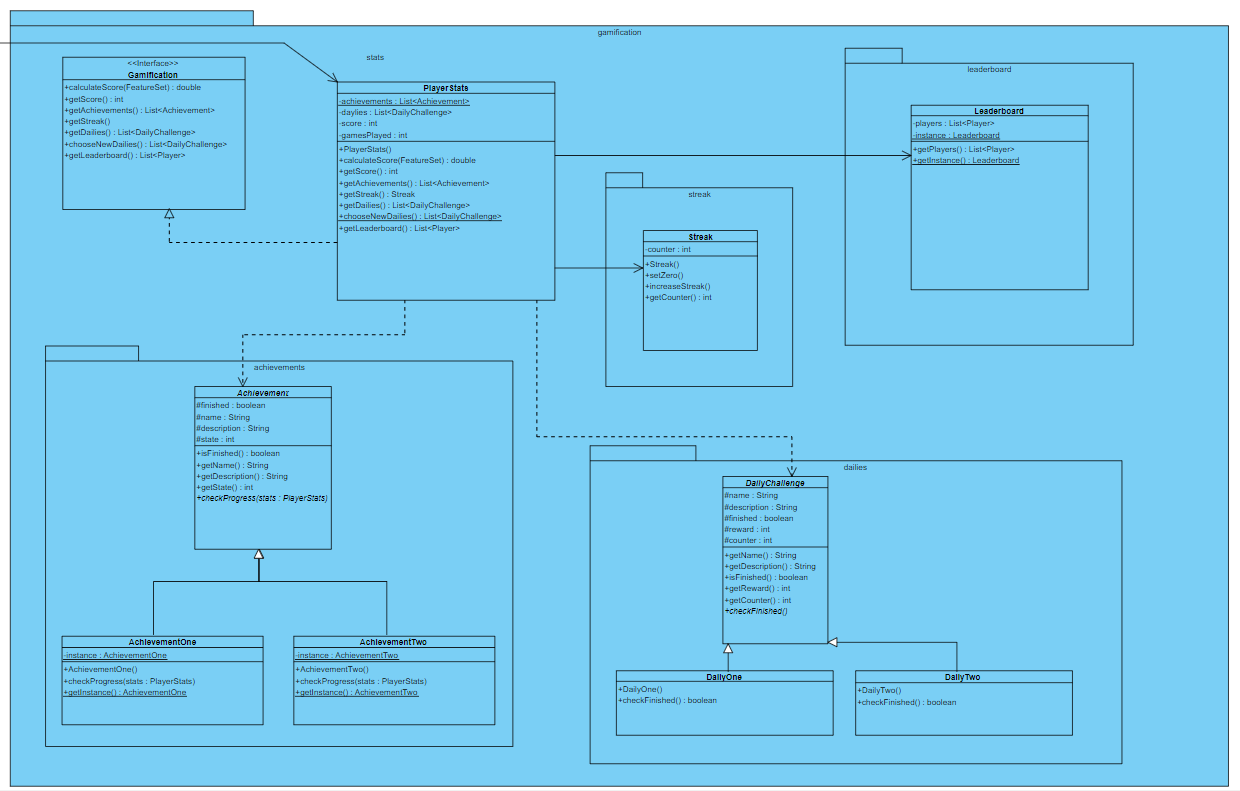
\includegraphics[width=\textwidth]{img/Gamification.PNG} \\
	
	Paket für die Gamification-Elemente. Zu den Gamification-Elementen gehören Punkte, Streak, Leaderboard, Achievements und Daily-Challenges.
	
	
	\subsection{Streak}
	Stellt eine Streak dar.
	
	\subsubsection{Streak}
	\begin{itemize}
		\item Beschreibung: Der Konstruktor einer Streak initialisiert den Zähler der Streak mit 0.
	\end{itemize}
	\subsubsection{setZero}
	\begin{itemize}
		\item Beschreibung: Setzt den Zähler der Streak auf den Wert 0 zurück.
	\end{itemize}
	\subsubsection{increaseStreak}
	\begin{itemize}
		\item Beschreibung: Erhöht den Zähler der Streak um den Wert 1.
	\end{itemize}
	\subsubsection{getCounter}
	\begin{itemize}
		\item Beschreibung: Gibt den aktuellen Zähler zurück.
		\item Rückgabewert: Der aktuelle Wert des Zählers.
	\end{itemize}
	
	
	\subsection{Leaderboard}
	Stellt ein Leaderboard dar. Es enthält eine Liste von Spielern.
	
	\subsubsection{getPlayers}
	\begin{itemize}
		\item Beschreibung: Gibt eine Liste von allen registrierten Spielern zurück.
		\item Rückgabewert: Liste von Spielern.
	\end{itemize}
	\subsubsection{getInstance}
	\begin{itemize}
		\item Beschreibung: Statische Methode. Sorgt dafür, dass nur ein LeaderBoard-Objekt existiert und gibt dieses zurück.
		\item Rückgabewert: Das LeaderBoard-Objekt.
	\end{itemize}
	
	Das Paket Dailies enthält eine abstrakte Klasse DailyChallenge, von der alle konkreten Daily-Challenges erben.
	
	\subsection{DailyChallenge}
	Die abstrakte Klasse DailyChallenge gibt an, wie Daily-Challenges aufgebaut sind. Lediglich die Methode checkFinished() ist abstrakt und muss von den Unterklassen implementiert werden.
	\subsubsection{getName}
	\begin{itemize}
		\item Beschreibung: Gibt den Namen der Daily-Challenge zurück.
		\item Rückgabewert: Ein String vom Namen der Daily-Challenge.
	\end{itemize}
	\subsubsection{getDescription}
	\begin{itemize}
		\item Beschreibung: Gibt die Beschreibung der Daily-Challenge zurück.
		\item Rückgabewert: Ein String von der Beschreibung der Daily-Challenge.
	\end{itemize}
	\subsubsection{isFinished}
	\begin{itemize}
		\item Beschreibung: Überprüft, ob die Aufgabe der Daily-Challenge an einem Tag schon erfüllt wurde.
		\item Rückgabewert: True, wenn die Aufgabe schon erfüllt ist, sonst false.
	\end{itemize}
	\subsubsection{setNotFinished}
	\begin{itemize}
		\item Beschreibung: Setzt den Wert der Variable finished auf false.
	\end{itemize}
	\subsubsection{getReward}
	\begin{itemize}
		\item Beschreibung: Gibt die Belohnung für das Abschließen einer Daily-Challenge zurück.
		\item Rückgabewert: Eine Punktzahl, die die Belohnung darstellt.
	\end{itemize}
	\subsubsection{getCounter}
	\begin{itemize}
		\item Beschreibung: Gibt den Wert des aktuellen Zählers zurück.
		\item Rückgabewert: Der Wert des aktuellen Zählers.
	\end{itemize}
	\subsubsection{checkFinished}
	\begin{itemize}
		\item Beschreibung: Überprüft, ob die Aufgabe der Daily-Challenge erfüllt ist.
		\item Parameter Das zugehörige PlayerStats-Objekt eines Spielers
		\item Rückgabewert: True, wenn die Aufgabe erfüllt ist, sonst false.
	\end{itemize}
	
	\subsection{DailyOne}
	Konkrete Implementierung der abstrakten Klasse DailyChallenge.
	\subsubsection{DailyOne}
	\begin{itemize}
		\item Beschreibung: Der Konstruktor von DailyOne setzt Namen und Beschreibung von DailyOne sowie die Belohnung. Der Zähler wird auf 0 gesetzt und finished auf false.
	\end{itemize}
	\subsubsection{checkFinished}
	%Konkret
	
	\subsection{DailyTwo}
	Konkrete Implementierung der abstrakten Klasse DailyChallenge.
	\subsubsection{DailyTwo}
	\begin{itemize}
		\item Beschreibung: Der Konstruktor von DailyTwo setzt Namen und Beschreibung von DailyTwo sowie die Belohnung. Der Zähler wird auf 0 gesetzt und finished auf false.
	\end{itemize}
	\subsubsection{checkFinished}
	%Konkret
	
	Das Paket Achievements enthält eine abstrakte Klasse Achievement, von der alle konkreten Achievements erben. \\
	Für ein Achievement gibt es im Gegensatz zu Anforderung /F750/ aus dem Pflichtenheft \textbf{keine} Punkte als Belohnung für das Abschließen.
	
	\subsection{Achievement}
	%\subsubsection{isFinished}
	%\begin{itemize}
	%\item Beschreibung: Überprüft, ob die Aufgabe des Achievements %erfüllt ist.
	%\item Rückgabewert: True, wenn die Aufgabe erfüllt ist, sonst false.
	%\end{itemize}
	\subsubsection{getName}
	\begin{itemize}
		\item Beschreibung: Gibt den Namen des Achievements zurück.
		\item Rückgabewert: Ein String vom Namen des Achievements.
	\end{itemize}
	\subsubsection{getDescription}
	\begin{itemize}
		\item Beschreibung: Gibt die Beschreibung des Achievements zurück.
		\item Rückgabewert: Ein String von der Beschreibung des Achievements.
	\end{itemize}
	\subsubsection{getState}
	\begin{itemize}
		\item Beschreibung: Gibt den aktuellen Zustand des Achievements zurück.
		\item Rückgabewert: Eine Zahl, die den aktuellen Zustand des Achievements darstellt.
	\end{itemize}
	\subsubsection{checkProgress}
	\begin{itemize}
		\item Beschreibung: Überprüft, ob die Aufgabe des Achievements erfüllt ist und setzt dementsprechend den Zustand des Achievements.
	\end{itemize}
	
	\subsection{AchievementOne}
	\subsubsection{AchievementOne}
	\begin{itemize}
		\item Beschreibung: Der Konstruktor von DailyTwo setzt Namen und Beschreibung von AchievementOne sowie den Zustand auf den entsprechenden Wert.
	\end{itemize}
	\subsubsection{checkProgress}
	%Konkret
	\subsubsection{getInstance}
	\begin{itemize}
		\item Beschreibung: Statische Methode. Sorgt dafür, dass nur ein AchievementOne-Objekt existiert und gibt dieses zurück.
		\item Rückgabewert: Das AchievementOne-Objekt.
	\end{itemize}
	
	\subsection{AchievementTwo}
	\subsubsection{AchievementTwo}
	\begin{itemize}
		\item Beschreibung: Der Konstruktor von DailyTwo setzt Namen und Beschreibung von AchievementTwo sowie den Zustand auf den entsprechenden Wert.
	\end{itemize}
	\subsubsection{checkProgress}
	%Konkret
	\subsubsection{getInstance}
	\begin{itemize}
		\item Beschreibung: Statische Methode. Sorgt dafür, dass nur ein AchievementTwo-Objekt existiert und gibt dieses zurück.
		\item Rückgabewert: Das AchievementTwo-Objekt.
	\end{itemize}
	
	
	\subsection{Gamification}
	Die Schnittstelle Gamification abstrahiert von der konkreten Implementierung von Gamification-Elementen und gibt dabei zu implementierende Methoden vor.
	\subsubsection{calculateScore}
	\begin{itemize}
		\item Beschreibung: Berechnet aus gegebenem Wert eine entsprechende Punktzahl für den Spieler.
		\item Parameter: Double, ein Wert zwischen 0 und 1. 
		\item Rückgabewert: Die berechnete erreichte Punktzahl des Spielers, eine natürliche Zahl.
	\end{itemize}
	\subsubsection{getScore}
	\begin{itemize}
		\item Beschreibung: Gibt die aktuelle Punktzahl des Spielers zurück.
		\item Rückgabewert: Die aktuelle Punktzahl des Spielers.
	\end{itemize}
	\subsubsection{getAchievements}
	\begin{itemize}
		\item Beschreibung: Gibt die aktuelle Achievements des Spielers zurück.
		\item Rückgabewert: Die aktuelle Achievements des Spielers in einer Liste.
	\end{itemize}
	\subsubsection{getStreak}
	\begin{itemize}
		\item Beschreibung: Gibt die aktuelle Streak des Spielers zurück.
		\item Rückgabewert: Die Streak des Spielers.
	\end{itemize}
	\subsubsection{getDailies}
	\begin{itemize}
		\item Beschreibung: Gibt die Daily-Challenges des Spielers zurück.
		\item Rückgabewert: Eine Liste der Daily-Challenges des Spielers.
	\end{itemize}
	\subsubsection{chooseNewDaily}
	\begin{itemize}
		\item Beschreibung: Statische Methode. Wählt für einen neuen Tag eine Daily-Challenge für alle Spieler gleich aus.
		\item Rückgabewert: Die Daily-Challenge des heutigen Tages.
	\end{itemize}
	\subsubsection{getLeaderboard}
	\begin{itemize}
		\item Beschreibung: Gibt eine Liste, die alle Spieler enthält.
		\item Rückgabewert: Liste aus Spielern, die das Leaderboard darstellen.
	\end{itemize}
	
	
	\subsection{PlayerStats}
	Die Klasse PlayerStats implementiert die Schnittstelle Gamification und regelt das Zusammenwirken der Gamification-Elemente und berechnet dabei die Punkte eines Spielers.
	\subsubsection{PlayerStats}
	Der Konstruktor von PlayerStats initialisiert den Punktestand mit 0 und lädt sich die verfügbaren Achievements und Daily-Challenges.
	\subsubsection{calculateScore}
	\subsubsection{getScore}
	\subsubsection{getAchievements}
	\subsubsection{getStreak}
	\subsubsection{getDailies}
	\subsubsection{chooseNewDaily}
	\subsubsection{getLeaderboard}
	\subsection{getRoundsPlayed}
	\begin{itemize}
		\item Beschreibung: Gibt die Anzahl der gespielten Runden eines Spielers zurück.
		\item Rückgabewert: Die Anzahl der gespielten Runden.
	\end{itemize}
	
	
	
	
	\chapter{Front-End}
	Es wird pro Art der Seite eine Haupt-Seite geben, die dann über die REST-API mit nutzerspezifischen Inhalten gefüllt werden.
	Hauptseiten:
	\begin{itemize}
		\item   Anmeldung
		\item   Organisator-Übersicht
		\item   Spielerstellung
		\item   Spieler-Übersicht
		\item   Spiel
	\end{itemize}
	\chapter{Sequenzdiagramme}
	
	\chapter{Datenhaltung}
	
	\section{Ordnerstruktur}
    \subsection{WAR-Datei}
        In der WAR-Datei\footnote{Für eine genauere Beschreibung wird auf die \href{https://tomcat.apache.org/tomcat-7.0-doc/appdev/deployment.html\#Standard\_Directory\_Layout}{Tomcat-Dokumentation} verwiesen.}, die in den \$CATALINA\_HOME Ordner von Tomcat gelegt wird, müssen folgende Ordner und Dateien existieren: 
    \begin{itemize}
        \item \texttt{*html, *jsp, etc.} Dies sind die statischen Datein, die direkt vom Browser später aufrufbar sein müssen. Sie können auch in untergeordneten Ordnern liegen.
        \item \texttt{/WEB-INF/web.xml} Dies ist die Web Application Deployment Descriptor Datei für die Anwendung. In dieser werden die Routen für Anfragen an den Server festgelegt.
        \item \texttt{/WEB-INF/classes/} Hier liegen die Klassen des Produktes mit ihrer Paketstruktur.
        \item \texttt{/WEB-INF/lib/} Hier liegen alle 3rd-Party Bibliotheken etc. 
    \end{itemize}
	
	\section{Konfiguration}
	Die Konfigurationsdatei enthält alle Einstellungsmöglichkeiten die das Produkt betreffen in der folgenden Form:
	\begin{itemize}
		\item organiserpassword (Das Passwort das ein Organisator bei der Registrierung angeben muss)
		\item mlserverurl       (Die URL unter der der ML-Server zu erreichen ist)
		\item homedirectory     (Das Verzeichnis unter dem Daten auf der Festplatte abgelegt werden sollen)
		\item database          (Kategorie für die Datenbankeinstellungen)
		\begin{itemize}
			\item type          (Typ der zu verwendenden Datenbank, Standard mysql)
			\item hostname      (Hostname unter dem der Datenbankserver erreichbar ist)
			\item port          (Port des Datenbankservers)
			\item username      (Nutzername des Datenbankbenutzers)
			\item password      (Passwort des Datenbankbenutzers)
		\end{itemize}
	\end{itemize}
	\section{Datenbank}
	In der Datenbank werden sämtliche spielrelevanten Daten gesichert.
	Die Standardimplementierung verwendet eine Mysql-Datenbank mit folgender geplanter Strukturierung der Daten.
	das Produkt verwendet eine Datenbank für seine Daten (fortan Hauptdatenbank genannt) sowie für jedes Spiel eine vom Organisator angegebene Datenbank.
	\subsection{Spielerdaten}
	Eine Tabelle in der Hauptdatenbank hält die Daten für die Spieler.
	Die einzelnen Spalten sind dabei die Folgenden:
	\begin{itemize}
		\item ID
		\item Username
		\item E-Mail-Addresse
		\item Passwort-Hash
		\item Passwort-Salt
		\item Score (Gesamt erreichte Punkte des Spielers)
		\item Anzahl gespielter Spiele
	\end{itemize}
	\subsection{Organisatordaten}
	Eine weitere Tabelle in der Hauptdatenbank hält die Daten der Organisatoren.
	Die einzelnen Spalten sind dabei die Folgenden:
	\begin{itemize}
		\item ID
		\item Username
		\item E-Mail-Addresse
		\item Passwort-Hash
		\item Passwort-Salt
	\end{itemize}
	Weiterhin wird jedem Organisator der Spieleinstellungen sichert eine weitere Tabelle mit seinen Spieleinstellungen zugeordnet.
	\begin{itemize}
		\item Titel des Pattern
		\item Beschreibung
		\item Art der Spielterminierung
		\item Spielmodus
		\item Eingeladene Spieler
	\end{itemize}
	\subsection{Merkmalsdatensätze}
	Jeder Merkmalsdatensatz erhält eine eigene Tabelle mit folgenden Inhalten:
	\begin{itemize}
		\item Dataset-Feature (Interner Name des Features)
		\item Englischer Name
		\item Englische Beschreibung
		\item Deutscher Name
		\item Deutsche Beschreibung
	\end{itemize}
	Die zum Merkmalsdatensatz gehörigen Graphen werden auf der Festplatte in einem Verzeichnis gespeichert.
	\subsection{Spieldaten}
	Die grundlegenden Daten zum Spiel werden in einer Tabelle in der Hauptdatenbank verwaltet.
	\begin{itemize}
		\item Titel
		\item Beschreibung
		\item Datenbankname
		\item Terminierungsstatus
		\item Spielmodus
	\end{itemize}
	Jedem Spiel wird vom Organisator eine eigene Datenbank zugewiesen.
	Löscht ein Organisator ein Spiel wird lediglich dessen Eintrag in voriger Tabelle gelöscht.
	Die spieleigene Datenbank bleibt unverändert.
	Jedes Spiel besitzt eine Tabelle die die Runden wie folgt hält.
	\begin{itemize}
		\item Zeitpunkt zu der die Runde gespielt wurde
		\item Name des Spielers der die Runde gespielt hat
		\item Anzahl der Teilrunden
		\item Vorhersagequalität
		\item Für die Runde erhaltene Punkte
		\item Ausgewählte Merkmale
		\item Optional: Als unwichtig markierte Merkmale
	\end{itemize}
	Weiterhin besitzt jedes Spiel je eine Tabelle, die die eingeladenen sowie die spielenden Spieler hält.
	
	
	
\end{document}
